\section{Il cubismo}
Il cubismo fu una delle correnti più innovative del '900. Nacque a Parigi intorno al 1907 per opera di Pablo Picasso e Georges Braque. Come punto di riferimento il cubismo prende spunto dall'attenta osservazione della pittura di Cézanne e del suo modo di rappresentare la natura scomponendola in forme geometriche elementari e sia sulla conoscenza dell'arte primitiva.

Il soggetto rappresentato è visto da più punti di osservazione contemporaneamente; l'immagine viene smontata nelle sue parti essenziali, analizzata dalle diverse angolazioni e poi riassemblata. In questo modo i cubisti introdussero il concetto di quarta dimensione: il tempo dell'osservazione.

Gli studiosi individuarono tre fasi del movimento cubista:
\begin{itemize}
  \item Cubismo formativo, caratterizzato da una progressiva deformazione e semplificazione dei volumi;
  \item Cubismo analitico, che si caratterizza per la frantumazione del soggetto in elementi così piccoli da renderne difficile il riconoscimento;
  \item Cubismo sintetico, si caratterizza per una rappresentazione più diretta e immediata della realtà dando spazio nei quadri cubisti a scritte e ai "papier collès", ovvero frammenti, incollati sulla tela, di giornali, carte da parati, carte da gioco e frammenti di legno. Il cubismo sintetico rivoluziona il concetto stesso di quadro portandolo ad essere esso stesso "realtà" e non "la rappresentazione della realtà"
\end{itemize}

\section{Pablo Picasso}
Nato a Malaga, in Spagna, nel 1881 Pablo Picasso si trasferì nel 1900 a Parigi dove entrò in contatto con l'ambiente intellettuale.

Le sue prime opere hanno per soggetto la vita degli emarginati e la vita del circo; la svolta si ha nel 1907 qunado la sia opera Les Demoisseles d'Avignon segna la nascita del cubismo. Durante la sua esistenza realizzò un gran numero di opere utilizzando diverse tecniche e stili. La figura di Picasso è importante anche per l'impegno civile dimostrato con il celebre dipinto Guernica.

\section{La Guernica}

\noindent
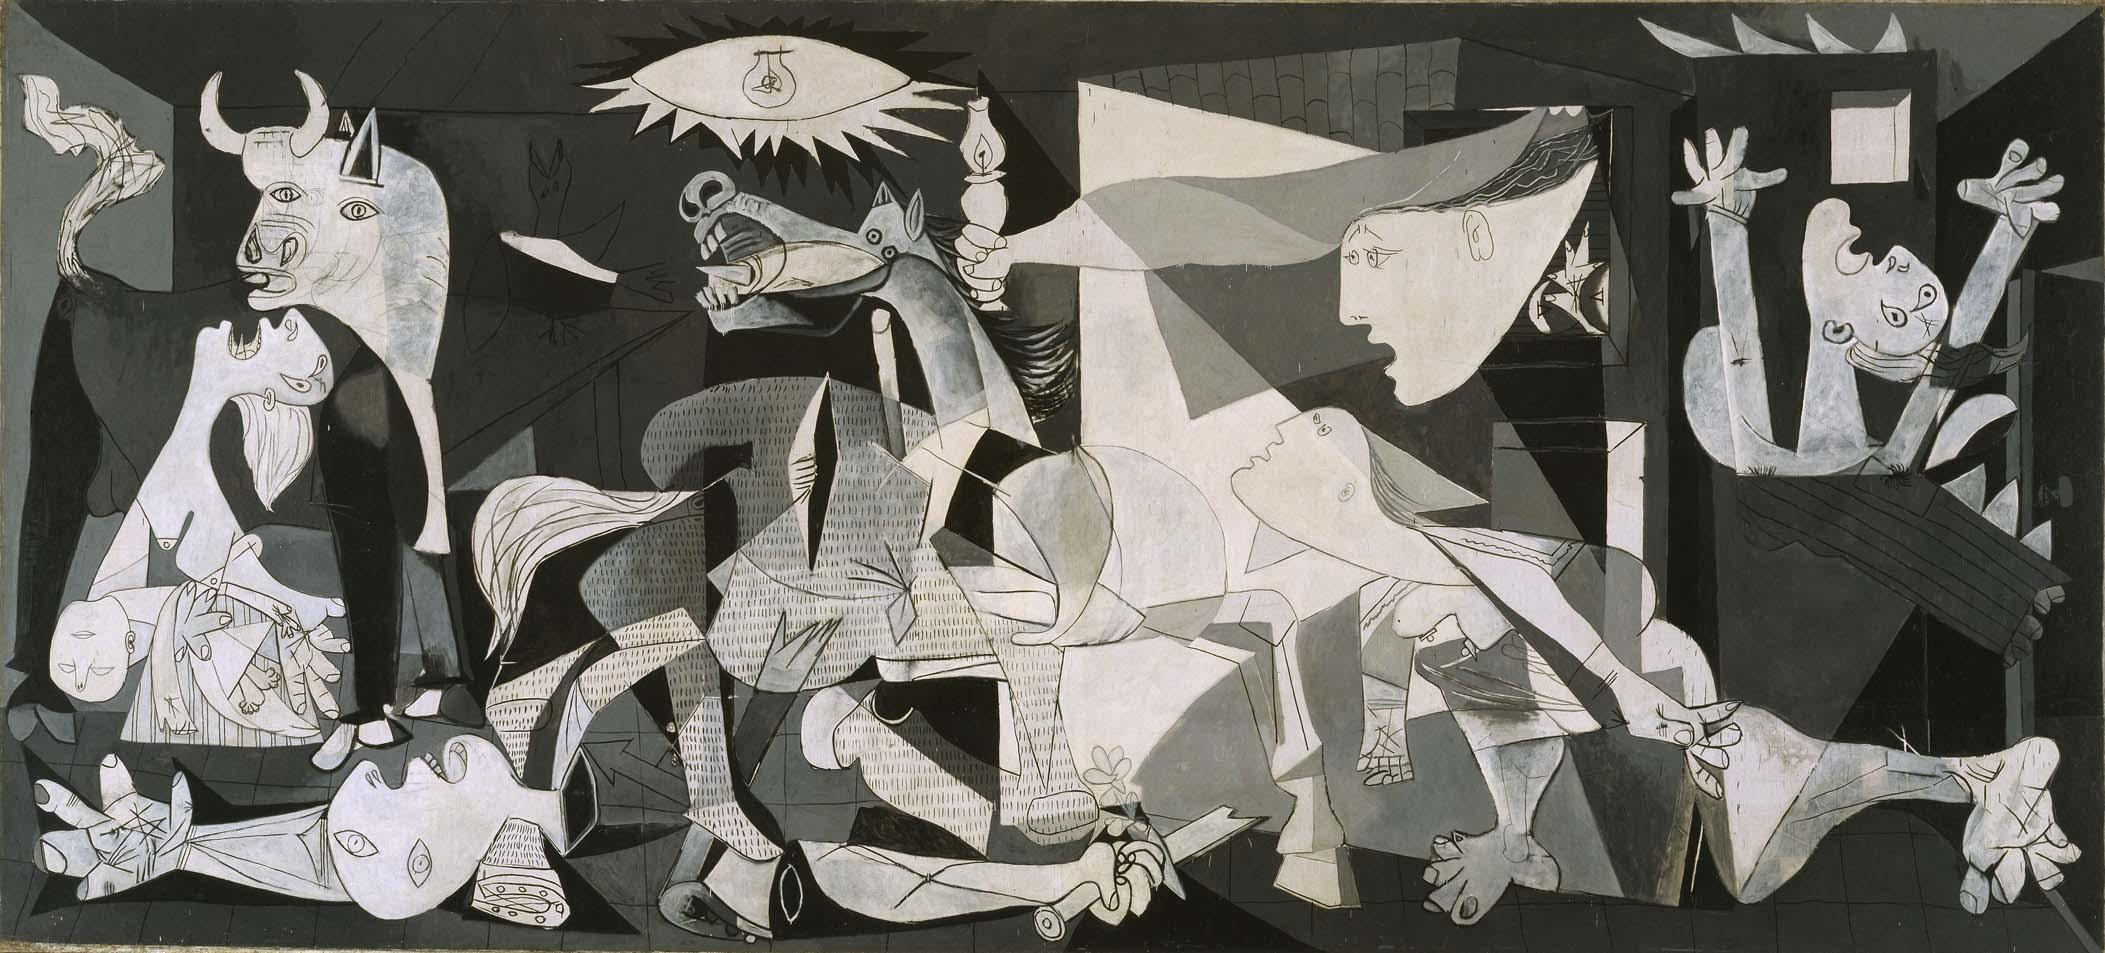
\includegraphics[width=\textwidth]{guernica.jpg}

Guernica era una piccola città della Spagna rasa al suolo nel 1937 da un bombardamento tedesco. Picasso decise di commemorare la strage dipingendo una grande tela per l'Esposizione Universale di Parigi del 1937. L'opera si basa su una costruzione piramidale in cima alla quale si trova un cavallo ferito che simboleggia la sofferenza del popolo spagnolo. Al vertice della composizione ci sono una luce elettrica e una lampada a olio, simboli della verità che trionfa sulla menzogna; sulla sinistra del quadro c'è un toro simbolo di forza. In basso a sinistra c'è l'immagine di una donna straziata dal dolore per la perdita del figlio; in alto a destra è raffigurata una donna con le braccia verso il cielo mentre la sua casa prende fuoco; in basso giace un soldato che impugna una spada sulla quale è nato un fiore simbolo di speranza.

Nella sua opera Picasso non vuole solo rappresentare la guerra di Guernica ma rappresenta la distruzione a cui porta il regime totalitario sollecitando tutti gli intellettuali e le forze popolari a schierarsi in difesa della libertà.
